\section{Investigating User-mode Networking}
\label{sec:trace}

The results in Figure \ref{fig:timing_large} led us to investigate why user-mode networking incurs such a large delay over bridged networking.
We traced the control path for packets going from a guest VM out to the network as well as from the network to a guest VM under both networking modes.
We focus on packets going from the guest to the network since this path incurs the largest overhead in the system.
The path from the network to the guest is detailed in the Appendix. 
We chose the RealTek 8139 driver because it is fully emulated by the system (unlike the paravirtualized virtio driver) and thus incurs the largest amount of delay.
The RTL8139 driver is also one of the most widely supported drivers and is the default for user-mode networking when the user does not specify an explicit configuration.
While Figure \ref{fig:timing_large} clearly shows a difference in performance between the drivers, the distinction between the different modes of networking was through the use of SLiRP and not specific to the driver.
%
%We were particularly interested because this is the default network configuration in KVM+QEMU if a user does not specify a configuration explicitly. 
%It is likely the default because the RTL8139 is widely supported, and because users will not be able to use bridged networking if they cannot set up a TAP device on their machine, a process that requires root access. 
%Because of that, it is most likely to be accessible, but as we can see, is also the least performant.
%
%In order to determine where the bottlenecks are occurring using the RTL8139, we traced the code path of a packet from the guest's application layer through the guest network stack and QEMU network emulation code using \texttt{callgrind} and \texttt{gdb}. 
%We discuss the traces and relevant functions in the code path for the guest transmissions below. 
%We provide an outline of the traces involved in the guest's receive path in the Appendix, along with the code path followed by packets on the transmit side that are shared by both the user-mode and bridged code. 

\subsection{Transmission from a Guest to the Network}
\label{subsec:usermode}

The control flow of a packet is split into two parts.
The packet first travels through the networking stack of the guest VM, and then moves through code in QEMU that is shared by both user-mode and bridged networking.
Once QEMU determines which mode of networking is being used, the code paths diverge and the sources of the slowdown become evident.

\subsubsection{Shared Control Path}
\begin{figure*}[!ht]
	\centering
		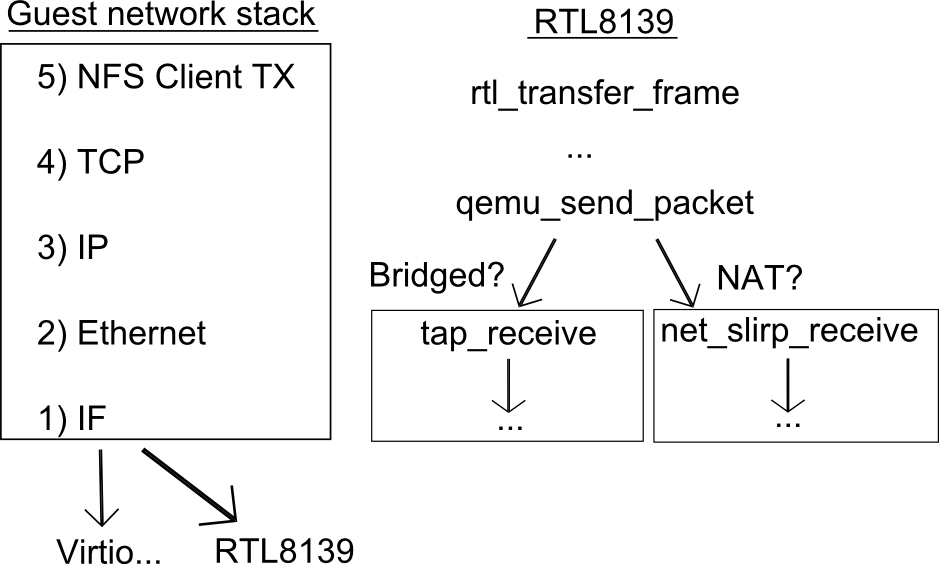
\includegraphics[scale=0.6]{codepath1}
	\caption{Virtualized client TX code path under bridged and user-mode (NAT) networking using the RTL8139 fully emulated driver. Both start at the top of the guest network stack, but diverge after \texttt{qemu\_deliver\_packet}.}
	\label{fig:codepath1}
\end{figure*}

Figure \ref{fig:codepath1} presents the code path originating at a guest VM's application layer.
The packet moves down the guest's networking stack to what it believes to be the physical network interface card.
At this point the packet is passed to whatever driver has been selected by the user.
In KVM+QEMU the options are \texttt{rtl8139}, \texttt{virtio}, or \texttt{e1000}.
Once the packet is processed by the driver, it encounters a sizeable amount of shared code (detailed in the Appendix) which is designed to determine which mode of networking is being used and passes the packet off to the
correct function.
If the guest is bridged then the packet is passed to \texttt{tap\_receive}, otherwise \texttt{net\_slirp\_receive} is invoked.

\begin{figure*}[!ht]
	\centering
		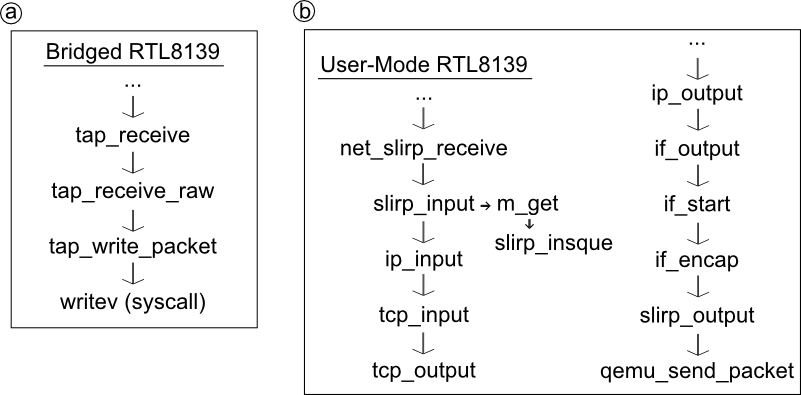
\includegraphics[scale=0.6]{codepath2_alt}
	\caption{Important functions in the divergent branches of bridged and user-mode networking.}
	\label{fig:codepath2}
\end{figure*}
\subsubsection{Bridged Packet Flow}
Figure \ref{fig:codepath2}a depicts the code path for bridged networking.
The code is relatively straight forward and concise.
\texttt{Tap\_receive} simply verifies the TAP state and then calls \texttt{tap\_receive\_raw}.
\texttt{Tap\_receive\_raw} translates the packet into iovectors.
\texttt{Tap\_write\_packet} is just a wrapper around the \texttt{writev} system call, checking the return value and error code.
Finally, \texttt{writev} writes the iovectors to the TAP.

\subsubsection{User-mode Packet Flow}

Figure \ref{fig:codepath2}b shows a flowchart of the user-mode networking path.
QEMU's SLiRP implementation, as you can see, requires considerably more code to process a packet compared to bridged networking.
The control flow starts when the RealTek driver passes the packet to the \texttt{net\_slirp\_receive} function.
\texttt{Net\_slirp\_receive} simply passes the packets along to \texttt{slirp\_input} along with the SLiRP connection state.
\texttt{Slirp\_input} calls two functions before the control flow continues: first to \texttt{m\_get}, which in turn calls \texttt{slirp\_insque}.
In \texttt{m\_get}, memory is allocated and then passed on to \texttt{slirp\_insque} which manages a free list of memory.
%The code attempts to reuse memory efficiently, but even with this optimization, we'll see that it still spends the majority of its time managing memory.
The chunk of memory is then returned to \texttt{slirp\_input} where the packet is then copied into the buffer.

Once the packet has been copied, it is passed ``up the stack'' to \texttt{ip\_input}. 
\texttt{Ip\_input} uses the IP headers to sanity check different aspects of the packet such as the checksum and length.
If for some reason the packet has been fragmented, it also attempts to reassemble it.
If the packet is found to be malformed then it is dropped and its memory is freed.

If the packet passes the tests in \texttt{ip\_input} it moves to \texttt{tcp\_input}.
\texttt{Tcp\_input} is a direct implementation of the TCP specification from September, 1981.
It does all the standard operations associated with TCP such as calculating the receive window and updating the TCP control block that QEMU maintains.
It then strips the guest's IP and TCP headers from the packet, leaving just the TCP payload, which is passed to \texttt{tcp\_output}.
It is at this point that the packet starts to move back ``down the stack'' to be put out onto the wire.
\texttt{Tcp\_output} handles TCP timers to determine when a packet should actually be sent.
Once a packet is cleared to send, the TTL and TOS fields are filled in and the packet is passed along.
With the transport layer complete the packet moves to \texttt{ip\_output} where its IP header fields are filled in with the host's information.
At this point the packet is fully formed.

It is handed off to \texttt{if\_output} which manages two different packet queues, \texttt{fastq} and \texttt{batchq}.
If a packet has the \texttt{IPTOS\_LOWDELAY} flag set, then it is placed on the \texttt{fastq}, which is intended for packets from an interactive application.
Otherwise, latency insensitive packets are placed on the \texttt{batchq}.
Each output queue is a doubly linked list of doubly linked lists of mbufs, each belonging to a separate socket.
This is intended to ensure that packets are fairly chosen for transmission across all the sockets of a system.
If a socket is found that does not have a linked list yet, then another is created.
To create the linked list, \texttt{if\_output} calls \texttt{m\_get} which, again, calls \texttt{slirp\_insque}.
The packet then moves on to \texttt{if\_start} which services both the \texttt{fastq} and the \texttt{batchq}.
As the names would indicate, the \texttt{fastq} is serviced first.
\texttt{If\_start} also cleans up the memory from each packet once the functions under it return.

Once a packet is chosen by \texttt{if\_start} it is passed to \texttt{if\_encap}.
Here the packet is prepared for going out on the wire by copying the packet header information into the appropriate header structs.
Finally, \texttt{slirp\_output} receives the packet which simply gives it to QEMU to be put on the wire through \texttt{qemu\_send\_packet}. 
%At this point qemu takes over and the rest of the control path is no longer dictated by the fact that usermode networking is in use.

\subsection{Code Path Timing}
\label{codePathTiming}
We timed the diverging sections of user-mode and bridged networking transmission paths. 
We began timing both paths at the function \texttt{rtl8139\_transfer\_frame}, ending the user-mode timing at \texttt{slirp\_output} and the bridged timing at \texttt{tap\_write\_packet}. 
The user-mode path took an average of 1.1 milliseconds, while the bridged path took an average of 44 microseconds, demonstrating a factor of 25 slowdown for user-mode networking relative to bridged.

\begin{figure}[htbp]
	\centering
		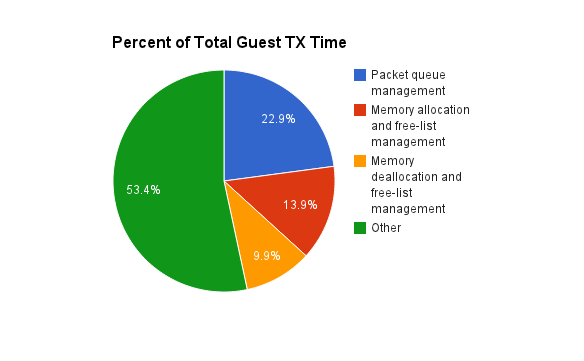
\includegraphics[scale=0.5]{usermodeTXtime}
	\caption{Almost half of the time spent in user-mode networking is spent in memory management.}
	\label{fig:usermodeTXtime}
\end{figure}

We then instrumented the SLiRP functions and found that almost 50\% of the overhead in user-mode networking is due to the memory management that takes place in \texttt{slirp\_input},
\texttt{m\_get}, \texttt{slirp\_insque}, \texttt{if\_output}, \texttt{if\_start}, \texttt{m\_free}, and \texttt{slirp\_remque}.
The most expensive of these functions was the management of the doubly linked lists of doubly linked lists of mbufs done in \texttt{if\_output} and \texttt{if\_start} which accounts for 22.9\%
of the transmit time.
Therefore, the management of memory was seen to be a major contributor to the slow down in user-mode networking.
Bridged networking does not have this problem since there is no need to manipulate the packet, which allows it to use the TAP to place the packet directly on the wire.

We also note that user-mode networking is essentially duplicating much of the work already done by the guest's network stack in order to rewrite the correct header fields to make the packet
look as though it originated from the host machine.
A packet must travel down the guest's networking stack, back up to the transport layer, and then back down before finally getting sent.


